With the JaLi language in place, this chapter will show how the \gls{mvu} architecture can be implemented using it. The button example will be continued, which is influenced by the Elm button example.

The program will have a model, that holds the current state of the program. The functions and types are expressed in listing \ref{mvu_types}. An update function defining how to handle each possible action, like \textit{Increment} and \textit{Decrement}. The last function \textit{view} is responsible of taking the model's value and transforming it to \gls{html} for the browser to render.
An \gls{adt} named \texttt{Msg} will hold the different actions that are possible. The \gls{html} structure can be represented by a \texttt{Node} type, which was explained in chapter \ref{jali}.
The \texttt{view} function takes the model and places into the \texttt{Tag} structure that is going to be the \gls{html} in the end but returns here just a structure of type \texttt{Node}. This can then be passed to \texttt{viewToHtml} which translates a value of type \texttt{Node} into a string of valid \gls{html}.

\begin{lstlisting}[columns=fullflexible, label={mvu_types}, language=Other, caption=Pseudo code to show functions and types]
type Node
type Msg
update: Msg -> Model -> Model
view: Model -> Node 

type Differ
diff: Node -> Node -> Differ
patch: Differ -> Node -> Node

patchToJs: Differ -> String
viewToHtml: Node -> String
\end{lstlisting}

An example implementation was shown in chapter \ref{jali}, but is presented again here for the ease of the reader. 

\lstinputlisting[label={jali_button_example2}, language=JaLi, caption=Button example written in JaLi]{./code/button.jali}

This implementation is enough to prepare one static view that can be rendered in the browser. By applying \texttt{viewToHtml} on the node we get the \gls{html} that has been saved to a file and displayed in the browser shown in figure \ref{fig:jali-button-in-browser}.

\begin{figure}
    \centering
    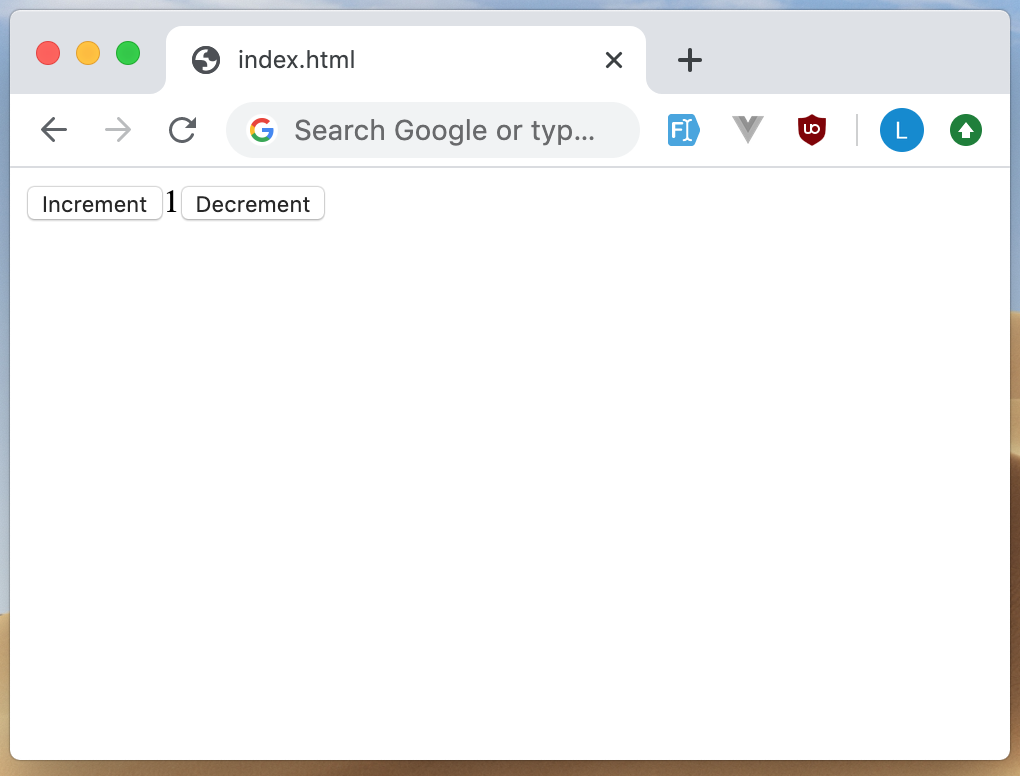
\includegraphics[width=0.8\textwidth]{./images/jali-button-in-browser}
    \caption{Initial view based on the JaLi implementation}
    \label{fig:jali-button-in-browser}
\end{figure}

To make the page dynamic it needs a \textit{handler}, attached to all the places where a user can interact with the website. For the button program this means to attach an on-click handler, that is triggered when the button is being clicked. The JaLi example listing \ref{jali_button_example2} shows that \texttt{update Increment} and \texttt{update Decrement} has been attached to the buttons. However, to make them actually work in the browser, all these actions need to be written in JavaScript, the only dynamic language the browser understands. This can be achieved by implementing a JaLi to JavaScript compiler, that translates the JaLi code into JavaScript. This has not been implemented, but it is very much possible, and thus we will simply simulate it by manual translation.

For the button example the actions \textit{Increment} and \textit{Decrement} alter the displayed value, by either incrementing its value or decrementing by one.
To make this as generic as possible and adapt previous ideas like \gls{vdom} comparing, two functions will be implemented: \texttt{diff} and \texttt{patch}. These are also the functions that need to be translated to JavaScript and executed---with the update function---on every action.
The \texttt{diff} function detects changes between two views and the \texttt{patch} function takes these changes and patches them in the view that is being shown.

Constructing two different views in listing \ref{two_views} by calling the \texttt{view} function with 1 and 2 would---when given to the \texttt{diff} function---return the \texttt{Differ} from listing \ref{non-reduced-differ}.

\begin{lstlisting}[columns=fullflexible, label={two_views}, language=JaLi, caption=Two views to compare]
view1 = Tag ('div') [] [
    Tag ('button') [] [Text ('Increment')],
    Tag ('p') [] [Text ((*@\textcolor{blue}{1}@*))],
    Tag ('button') [] [Text ('Decrement')],
];
view2 = Tag ('div') [] [
    Tag ('button') [] [Text ('Increment')],
    Tag ('p') [] [Text ((*@\textcolor{blue}{2}@*))],
    Tag ('button') [] [Text ('Decrement')],
];
\end{lstlisting}

Listing \ref{diff_function} shows the definition for the \texttt{diff} function. It receives two views and traverses through it, comparing always the first element in the list of nodes. If both \texttt{Tags} are the same it continues comparing, by using the helper function \texttt{fold} to iterate over the children nodes on the compared tags.
If it encounters a difference either on the \texttt{Tag} or on the \texttt{Text} it returns a \texttt{Change} constructor with the value from view2, since view2 is the newer view.
\texttt{fold} just takes the first element out of the list and calls \texttt{diff} on it again. If that call returns a \texttt{Change} it indicated that there is a change at that child by returning a \texttt{Path} with the index of the child. As a result, we get a \texttt{Path} to the child that must be changed. 
This function at this stage only detects the first difference on two views and then terminates. This is for the trivial button example sufficient but should be extended for real use.

\begin{lstlisting}[columns=fullflexible, label={non-reduced-differ}, language=Other, caption=Differ path detecting change on \texttt{Text} node]
$ Constant
(ADTValue
   ("Path","Differ",
    [IntegerValue (*@\textcolor{blue}{1}@*);
     ADTValue
       ("Path","Differ",
        [IntegerValue (*@\textcolor{blue}{0}@*);
         ADTValue
           ("Change","Differ",
             [ADTValue ("Text","Node",[IntegerValue (*@\textcolor{blue}{2}@*)])])
        ])]))
\end{lstlisting}

\lstinputlisting[columns=fullflexible, label={diff_function}, language=JaLi, caption=Diff function detecting changes on two views]{./code/diff.jali}

In order to apply this detected change, the \texttt{patch} function takes the old view, the changes and returns a new view.

\lstinputlisting[columns=fullflexible, label={patch_function}, language=JaLi, caption=Patch function applying changes on old view]{./code/patch.jali}

It does this by iterating over the \texttt{Differ} \gls{adt} held in \texttt{changes}, which is a recursive path structure that has a \texttt{Path} and \texttt{Change} constructor. When a \texttt{Change} is encountered it immediately returns the value from it, otherwise it will take the index from the \texttt{Path} and find the corresponding \texttt{Tag} node in the view and follow it recursively by calling patch again.
It uses two helper functions: \texttt{mapi} and the inner function called \texttt{f}. \texttt{mapi} iterates through a list a applies the given function on each element it passes while maintaining an index, that is passed to the function. This allows the tracking of elements in the view and the index from the \texttt{Path}.
Ultimately \texttt{patch} will then return an updated \texttt{Node} structure that looks like \texttt{view2} from listing \ref{two_views}.

By compiling the patch function to JavaScript, it can be executed in the browser, thus updating the right child in the actual view. One missing feature is to update the value of the model stored in the JavaScript in the browser. 

\paragraph{Generating JavaScript code from JaLi} In order to make the whole \gls{mvu} cycle work, a few additions needs to happen to the existing program. In principal when a button is clicked, the model needs to be either increased or decreased by one, a new view created with the updated model, the differences between the old and new view calculated and then applied on the old view, by only updating the changed part.

\begin{lstlisting}[columns=fullflexible, label={update_and_patch}, language=JaLi, caption=Update and patch on action]
func updateAndPatch action =
  oldModel = readGlobal ('model');
  newModel = update (action) (oldModel);
  eval (patchToJs (diff (view newModel) (view (oldModel))))
  setGlobal ('model') (newModel)
end
\end{lstlisting}

This function when compiled to JavaScript and executed would read from global variable called \texttt{model} the value, and update it accordingly to the action passed in. This \texttt{newModel} would then be used to construct a new view and compared by using \texttt{diff} and the old view.
The \texttt{update} and \texttt{diff} functions are written in JaLi and have been introduced previously. The new and crucial function is the \texttt{patchToJs} function. It is in essence the same as the \texttt{patch} function but generates optimized JavaScript code to handle the change.

The global reading of the variable is not shown here as this would be generated by the JavaScript compiler and so is the setting of the variable from line 5. Even though the \texttt{update} and \texttt{diff} functions are implemented they would also need to be compiled to JavaScript. The only part that is generating JavaScript that needs no further compiling is the result from the \texttt{patchToJs} function. It would be executed by the native implemented JavaScript function \textit{eval}\footnote{\url{https://developer.mozilla.org/en-US/docs/Web/JavaScript/Reference/Global_Objects/eval}}.

By evaluating the \texttt{patchToJs} function with the Path that was previously computed, we can compute the JavaScript needed to update the correct child. The \texttt{patchToJs} function elevates the complete \gls{dom} access, by using accessors like \textit{children} on \gls{dom} nodes to follow the \texttt{Differ} path down to the change.

\lstinputlisting[columns=fullflexible, label={patch_to_js_function}, language=JaLi, caption=Patch function generating JavaScript]{./code/patch-to-js.jali}

\begin{lstlisting}[columns=fullflexible, label={patch_to_js_result}, language=JaLi, caption=JavaScript that patches the view]
document.body.children[0].children[1].children[0].innerHTML = (*@\textcolor{blue}{2}@*);
\end{lstlisting}

\paragraph{JavaScript compiler} Now lacking the JaLi to JavaScript compiler does not stop us from compiling the code to JavaScript by hand. In theory and only able to do it manually this section shows how the JavaScript compiled program should look like.

To make the \gls{adt} functionality in JavaScript work, a class for the super-type of an \gls{adt} could be defined and the different constructors be classes that extend this class, with a constructor and fields for the different type arguments on an \gls{adt}.

\lstinputlisting[columns=fullflexible, label={adts_js}, language=JavaScript, caption=JavaScript code for ADTs and other types]{./code/mvu/adts.js}

The code in listing \ref{adts_js} also shows the global model variable.

The key part of the \gls{mvu} cycle in this case is the \texttt{updateAndPatch} function that is attached to the buttons and triggered by the \textit{onclick} event.

\lstinputlisting[columns=fullflexible, label={update_and_patch_js}, language=JavaScript, caption=JavaScript code for updateAndPatch]{./code/mvu/update-and-patch.js}

All the things previously described from the \texttt{updateAndPatch} now need to happen in JavaScript.

The \texttt{update} function in JavaScript is as trivial as it was before---just incrementing or decrementing the value.

\lstinputlisting[columns=fullflexible, label={update_js}, language=JavaScript, caption=Update function in JavaScript]{./code/mvu/update.js}

The result will then be used to build the two views, which are then compared.

\lstinputlisting[columns=fullflexible, label={view_js}, language=JavaScript, caption=View function in JavaScript]{./code/mvu/view.js}

\lstinputlisting[columns=fullflexible, label={diff_js}, language=JavaScript, caption=Diff function in JavaScript]{./code/mvu/diff.js}

\begin{figure}
    \centering
    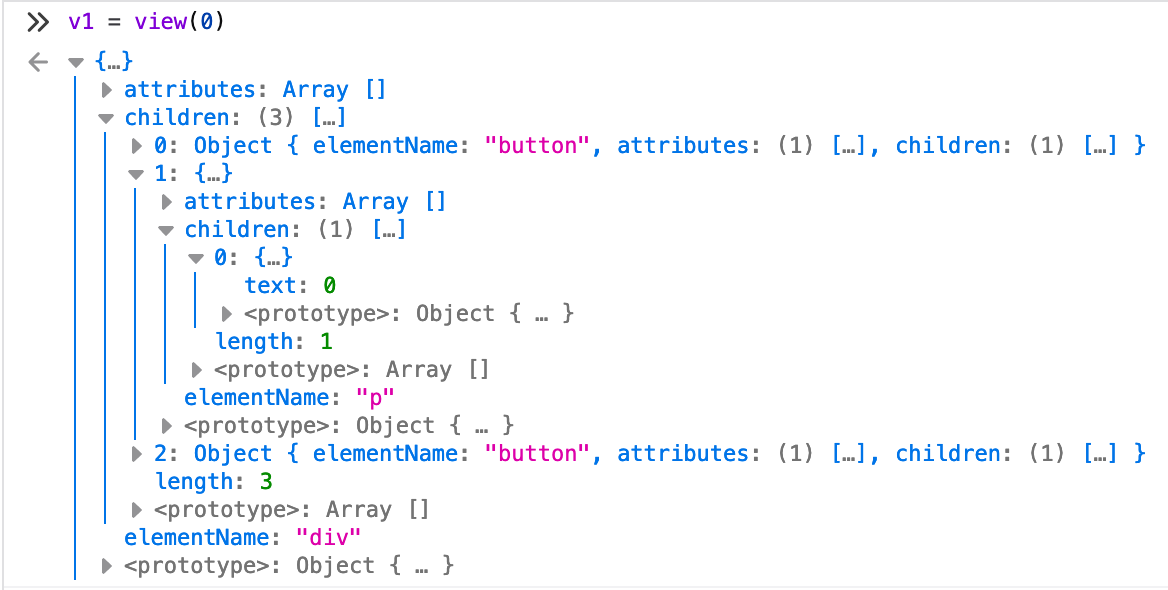
\includegraphics[width=0.8\textwidth]{./images/mvu-js-view}
    \caption{Constructing a view instance in JavaScript}
    \label{fig:view_js}
\end{figure}

\begin{figure}
    \centering
    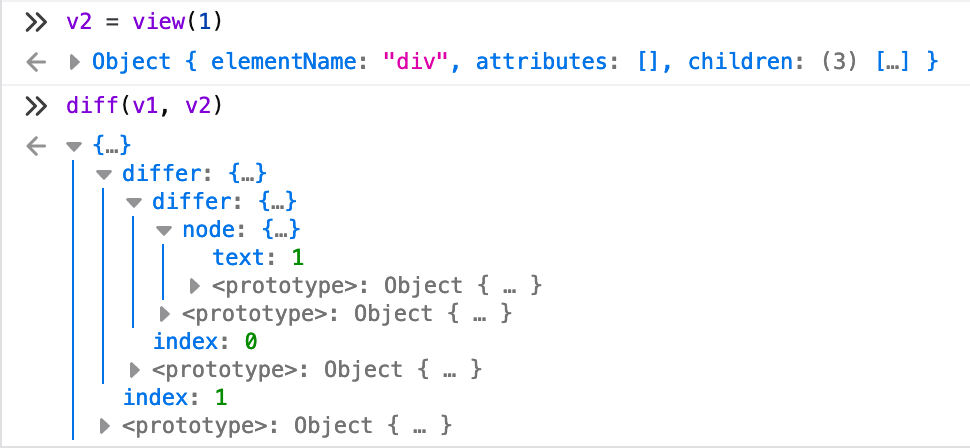
\includegraphics[width=0.8\textwidth]{./images/mvu-js-diff}
    \caption{Differ object after comparing \texttt{view(0)} and \texttt{view(1)} in JavaScript}
    \label{fig:view_js}
\end{figure}

Finally, the \texttt{patchToJs} function applies the changes and forces to rerender the parts in the \gls{dom}
, because the \texttt{patchToJs} is unchanged it returns a string of JavaScript code, that is then executed with the \texttt{eval} function.

\lstinputlisting[columns=fullflexible, label={patch_to_js_js}, language=JavaScript, caption=PatchToJs function in JavaScript]{./code/mvu/patch-to-js.js}

\begin{lstlisting}[columns=fullflexible, label={eval_patch_to_js_result}, language=JaLi, caption=Eval the JavaScript string that patches the view]
eval("document.body.children[0].children[1].children[0].innerHTML = (*@\textcolor{blue}{1}@*);");
\end{lstlisting}

\begin{figure}
    \centering
    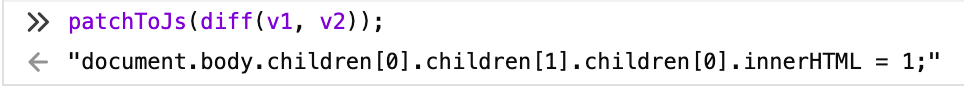
\includegraphics[width=0.8\textwidth]{./images/mvu-patch-result}
    \caption{Result JavaScript string from calling \texttt{patchToJs}}
    \label{fig:patch_result_js}
\end{figure}

\begin{figure}
    \centering
    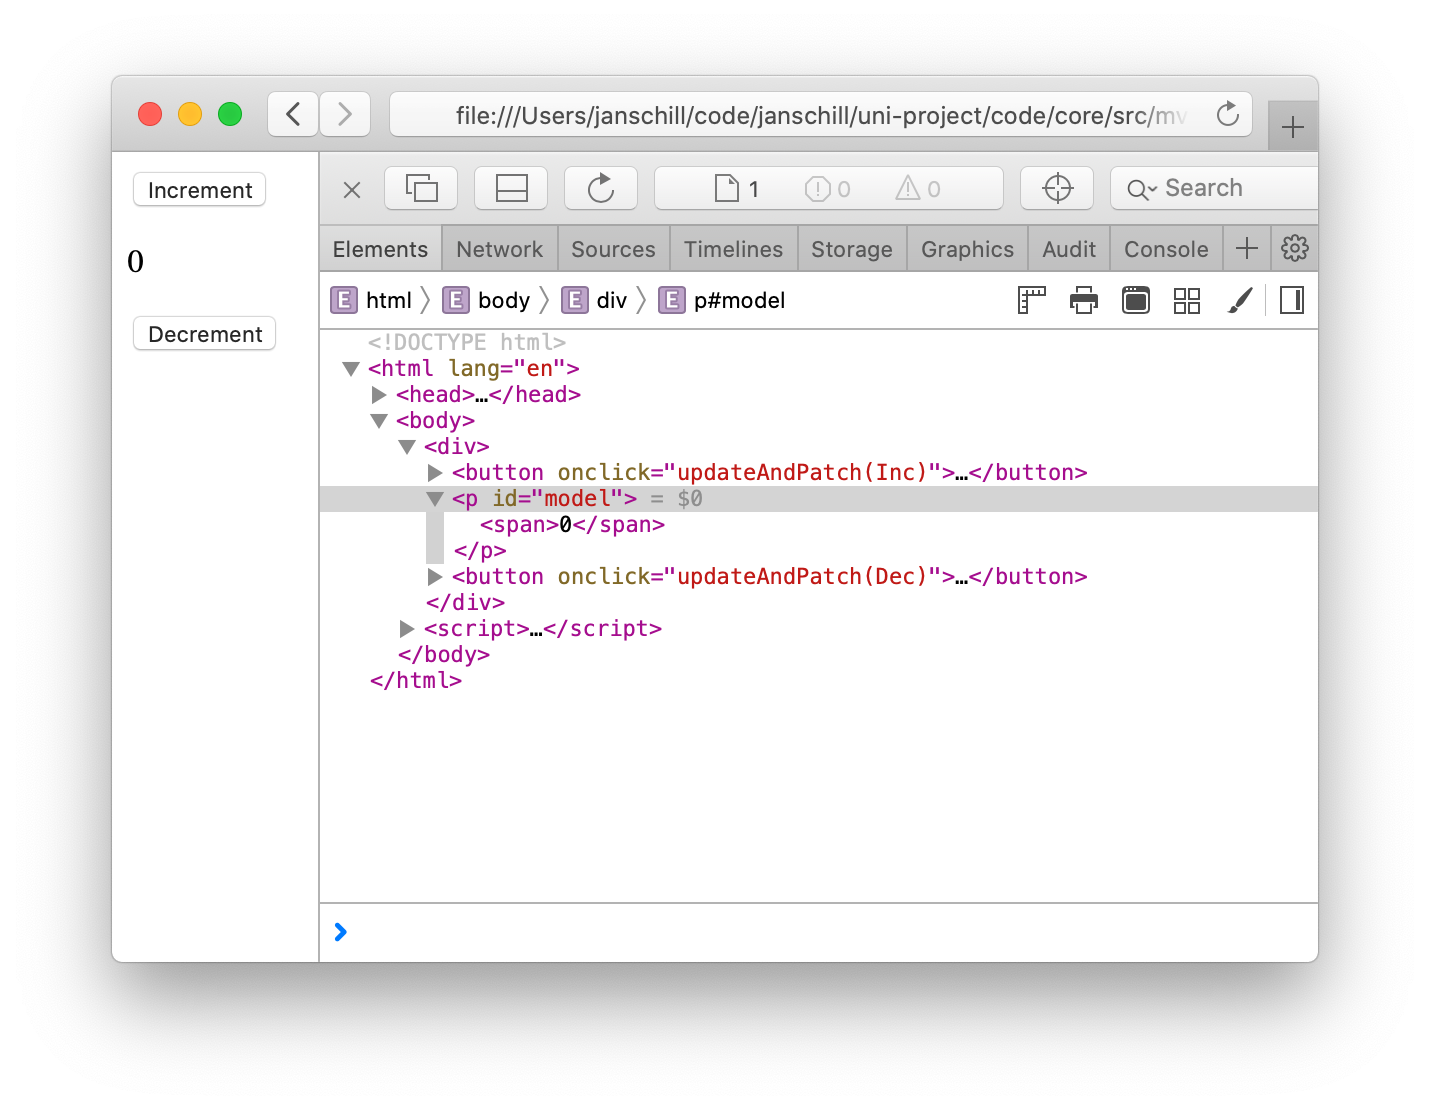
\includegraphics[width=0.8\textwidth]{./images/mvu-patch-js-1}
    \caption{Initial view}
    \label{fig:patch-1_js}
\end{figure}

\begin{figure}
    \centering
    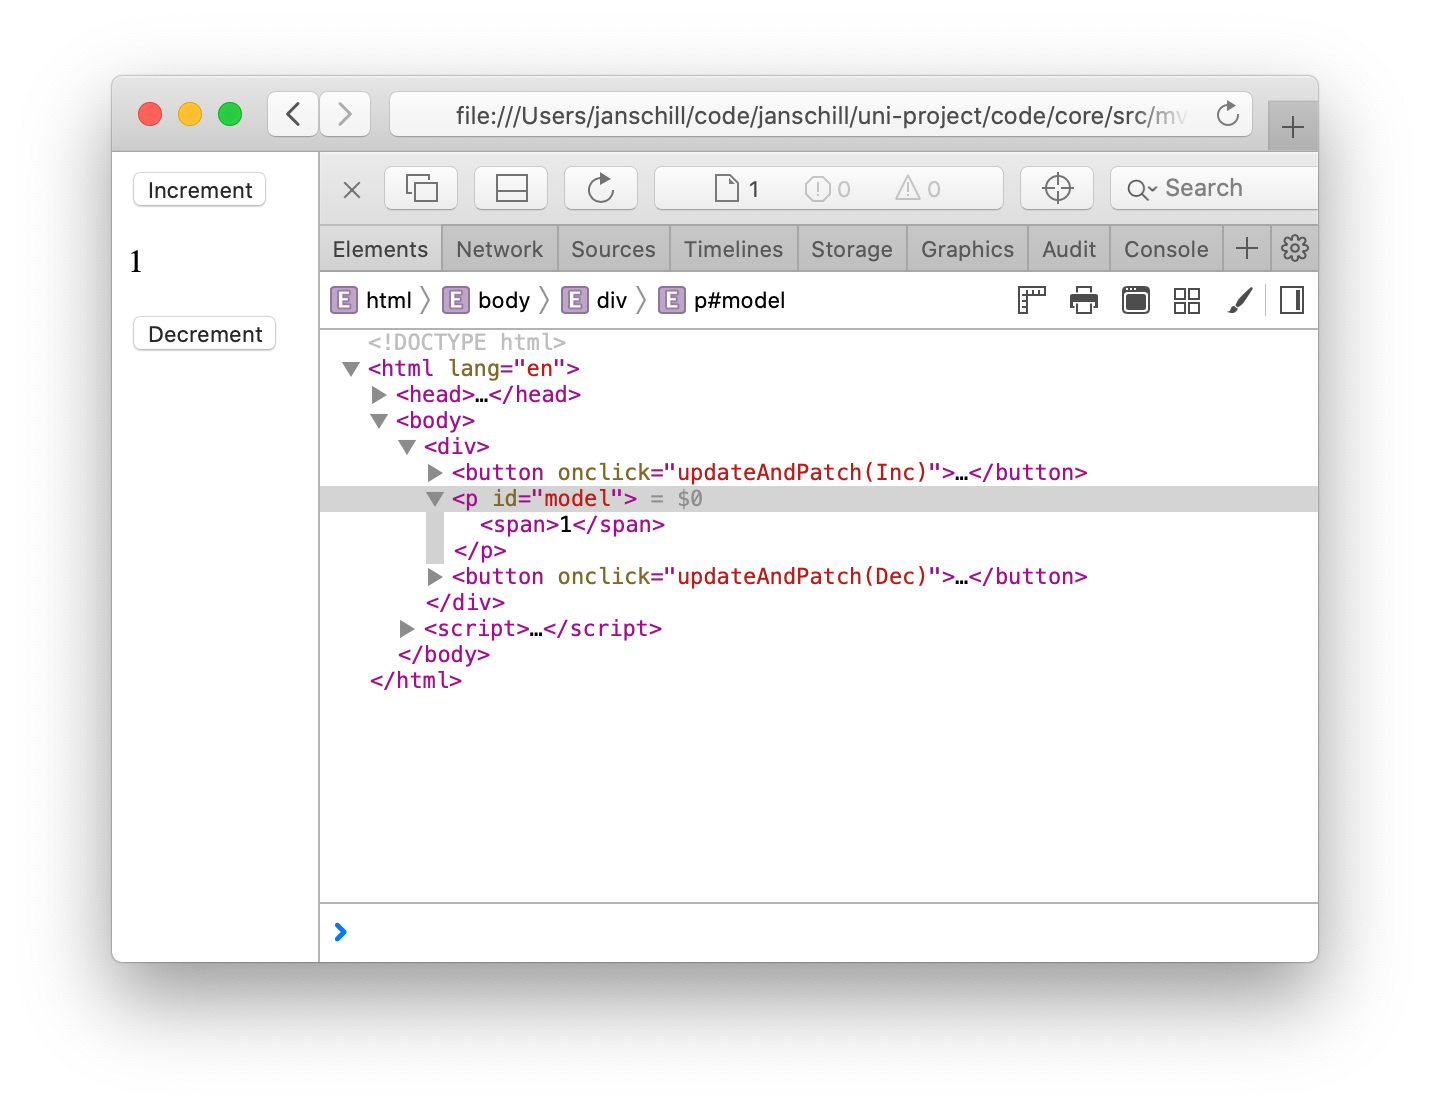
\includegraphics[width=0.8\textwidth]{./images/mvu-patch-js-2}
    \caption{View after clicking increment button}
    \label{fig:patch-2_js}
\end{figure}
